\documentclass[zihao=-4,fontset = none]{ctexart}
\usepackage{xeCJKfntef}
\newif\ifpad

% \usepackage[paperwidth=10cm,paperheight=16cm,textwidth=240bp,vmargin=0.25cm]{geometry}
% \pagestyle{empty}

% \usepackage[a4paper,textwidth=492bp,vmargin=2cm]{geometry}
\usepackage{mwe}
\usepackage{amssymb,amsmath,amsthm}
\usepackage{unicode-math}
\allowdisplaybreaks[4]
\usepackage{graphicx}
\usepackage{siunitx,physics}
\sisetup{inter-unit-product = \ensuremath { { } \cdot { } } }
\theoremstyle{definition}
\newtheorem*{solution}{解}
\usepackage{xpatch}
% \makeatletter
% \xpatchcmd{\@thm}{\thm@headpunct{:}}{\thm@headpunct{:}}{}{}
% \makeatother

% \setmainfont{Fira Sans}
% \setmathfont{Fira Math}

% \setmainfont{XITS}
% \setmathfont{XITS Math}
\xeCJKsetup{PunctStyle=kaiming}
% \setCJKmainfont[Mapping=fullwidth-stop]{Source Han Sans CN}

% \setCJKmainfont{Source Han Serif CN}[
%   UprightFont    = *-Regular,
%   BoldFont       = *-Bold,
%   ItalicFont     = 方正新楷体简体,
%   BoldItalicFont = *-Bold,
%   Mapping=fullwidth-stop
% ]



% \padtrue
\ifpad
\usepackage[paperwidth=11.5cm,paperheight=18.4cm,textwidth=22\ccwd,vmargin=0.5cm,marginparsep=0pt]{geometry}
\setmainfont{Fira Sans}
\setmathfont{Fira Math}
\usepackage{xunicode-addon}
\xeCJKDeclareCharClass{CJK}{%
  "24EA,        % ⓪
  "2460->"2473, % \textcircled{1}–⑳
  "3251->"32BF, % ㉑–㊿
  "24FF,        % ⓿
  "2776->"277F, % ❶–❿
  "24EB->"24F4  % ⓫–⓴
}
\xeCJKDeclareCharClass{Default}{"24EA, "2460->"2473, "3251->"32BF}
% \xeCJKDeclareCharClass{CJK}{%
%   "1F10B,        % ⓪
%   "2780->"2789, % \textcircled{1}–⑳
%   "3251->"32BF, % ㉑–㊿
%   "24FF,        % ⓿
%   "2776->"277F, % ❶–❿
%   "24EB->"24F4  % ⓫–⓴
% }
% \xeCJKDeclareCharClass{Default}{"1F10B, "2780->"2789, "3251->"32BF}

% 将中文字体声明为(西文)字体族
\newfontfamily\EnclosedNumbers{Source Han Sans CN}

% 放置钩子,只让带圈字符才需更换字体
\AtBeginUTFCommand[\textcircled]{\begingroup\EnclosedNumbers}
\AtEndUTFCommand[\textcircled]{\endgroup}

\setCJKmainfont[Mapping=fullwidth-stop]{Source Han Sans CN}
\setCJKsansfont{Source Han Sans CN}
\setCJKmonofont{仿宋}

\usepackage{tikz,pgf}
\usetikzlibrary{shapes,calc}
\makeatletter
\newcommand\thumb{%
  \begingroup
  \tikzpicture[remember picture,overlay]
      \node[fill=gray,text=black,anchor=north east,xshift=0.15mm,
            yshift=-2.8mm,
            shape=semicircle,shape border rotate=90,
            minimum height=5mm,minimum width=2.5mm,
            font=\tiny\bfseries]
        at (current page.north east)
        {\arabic{page}\hspace*{-0.5\ccwd}};
  \endtikzpicture
  \endgroup
  }
\makeatother
\setlength{\headheight}{15pt}
\usepackage{fancyhdr}
\pagestyle{fancy}
\fancyhf{}
\fancyhead[r]{\thumb}
\renewcommand{\headrulewidth}{0pt}
\renewcommand{\footrulewidth}{0pt}
% \def\kuo#1{\mbox{({#1})}}
\def\kuo#1{(\nobreak#1\nobreak)}
% \newcommand{\fivech}[4]{\noindent\begin{tabular}{*{5}{@{}p{0.2\textwidth}@{}}}{A}.#1 & {B}.#2 & {C}.#3 & {D}.#4 & {E}.#5\end{tabular}}
\newcommand{\fivech}[5]{\noindent\begin{tabular}{*{2}{@{}p{0.5\textwidth}@{}}}{A}.#1 & {B}.#2\end{tabular}\\\begin{tabular}{*{2}{@{}p{0.5\textwidth}@{}}}{C}.#3 & {D}.#4\end{tabular}\\\begin{tabular}{@{}p{\textwidth}@{}}{E}.#5\end{tabular}}
\makeatletter
\newcommand{\fourch}[4]{\noindent\begin{tabular}{*{4}{@{}p{0.25\textwidth}@{}}}\@hangfrom{A.}#1 & \@hangfrom{B.}#2 & \@hangfrom{C.}#3 & \@hangfrom{D.}#4\end{tabular}}
\makeatother
\newcommand{\twoch}[4]{\noindent\begin{tabular}{*{2}{@{}p{0.5\textwidth}@{}}}{A}.#1 & {B}.#2\end{tabular}\\\begin{tabular}{*{2}{@{}p{0.5\textwidth}@{}}}{C}.#3 & {D}.#4\end{tabular}}
\newcommand{\onech}[4]{\noindent{A}.#1 \\ {B}.#2 \\ {C}.#3 \\ {D}.#4}

\newcommand{\foursanch}[3]{\noindent\begin{tabular}{*{3}{@{}p{0.333\textwidth}@{}}}\textsf{A}.#1 & \textsf{B}.#2 & \textsf{C}.#3\end{tabular}}
\newcommand{\twosanch}[3]{\noindent\begin{tabular}{*{2}{@{}p{0.5\textwidth}@{}}}{A}.#1 & {B}.#2\end{tabular}\\\begin{tabular}{@{}p{\textwidth}@{}}{C}.#3\end{tabular}}
\newcommand{\onesanch}[3]{\noindent\textsf{A}.#1 \\ \textsf{B}.#2 \\ \textsf{C}.#3}
\newcommand{\dui}{\marginpar{(\nobreak{}对\nobreak{})}}
\newcommand{\cuo}{\marginpar{(\nobreak{}错\nobreak{})}}
\def\xiahua#1{\CJKunderline*[thickness=1pt, format=\color{red}]{#1}}
\else
\usepackage[a4paper,textwidth=41\ccwd,vmargin=2cm]{geometry}
\setmainfont{XITS}
\setmathfont{XITS Math}
\usepackage{xcolor}
\usepackage{xunicode-addon}
\xeCJKDeclareCharClass{CJK}{%
  "24EA,        % ⓪
  "2460->"2473, % \textcircled{1}–⑳
  "3251->"32BF, % ㉑–㊿
  "24FF,        % ⓿
  "2776->"277F, % ❶–❿
  "24EB->"24F4  % ⓫–⓴
}
\xeCJKDeclareCharClass{Default}{"24EA, "2460->"2473, "3251->"32BF}

% 将中文字体声明为(西文)字体族
\newfontfamily\EnclosedNumbers{Source Han Serif CN}

% 放置钩子,只让带圈字符才需更换字体
\AtBeginUTFCommand[\textcircled]{\begingroup\EnclosedNumbers}
\AtEndUTFCommand[\textcircled]{\endgroup}

\setCJKmainfont{Source Han Serif CN}[
  UprightFont    = *-Regular,
  BoldFont       = *-Bold,
  ItalicFont     = 方正新楷体简体,
  BoldItalicFont = *-Bold,
  Mapping=fullwidth-stop
]
\setCJKsansfont{Source Han Sans CN}
% \def\kuo#1{\mbox{(\textsf{#1})}}
\def\kuo#1{(\nobreak\textsf{#1}\nobreak)}
% \newcommand{\fivech}[4]{\noindent\begin{tabular}{*{5}{@{}p{0.2\textwidth}@{}}}{A}.#1 & {B}.#2 & {C}.#3 & {D}.#4 & {E}.#5\end{tabular}}
\newcommand{\fivech}[5]{\noindent\begin{tabular}{*{2}{@{}p{0.5\textwidth}@{}}}{A}.#1 & {B}.#2\end{tabular}\\\begin{tabular}{*{2}{@{}p{0.5\textwidth}@{}}}{C}.#3 & {D}.#4\end{tabular}\\\begin{tabular}{@{}p{\textwidth}@{}}{E}.#5\end{tabular}}
% \newcommand{\fourch}[4]{\noindent\begin{tabular}{*{4}{@{}p{0.25\textwidth}@{}}}\textsf{A}.#1 & \textsf{B}.#2 & \textsf{C}.#3 & \textsf{D}.#4\end{tabular}}
\makeatletter
\newcommand{\fourch}[4]{\noindent\begin{tabular}{*{4}{@{}p{0.25\textwidth}@{}}}\@hangfrom{\textsf A.}#1 & \@hangfrom{\textsf B.}#2 & \@hangfrom{\textsf C.}#3 & \@hangfrom{\textsf D.}#4\end{tabular}}
\makeatother
\newcommand{\twoch}[4]{\noindent\begin{tabular}{*{2}{@{}p{0.5\textwidth}@{}}}\textsf{A}.#1 & \textsf{B}.#2\end{tabular}\\\begin{tabular}{*{2}{@{}p{0.5\textwidth}@{}}}\textsf{C}.#3 & \textsf{D}.#4\end{tabular}}
\newcommand{\onech}[4]{\noindent\textsf{A}.#1 \\ \textsf{B}.#2 \\ \textsf{C}.#3 \\ \textsf{D}.#4}

\newcommand{\foursanch}[3]{\noindent\begin{tabular}{*{3}{@{}p{0.333\textwidth}@{}}}\textsf{A}.#1 & \textsf{B}.#2 & \textsf{C}.#3\end{tabular}}
\newcommand{\twosanch}[3]{\noindent\begin{tabular}{*{2}{@{}p{0.5\textwidth}@{}}}\textsf{A}.#1 & \textsf{B}.#2\end{tabular}\\\begin{tabular}{@{}p{\textwidth}@{}}\textsf{C}.#3\end{tabular}}
\newcommand{\onesanch}[3]{\noindent\textsf{A}.#1 \\ \textsf{B}.#2 \\ \textsf{C}.#3}
\newcommand{\dui}{\marginpar{(\nobreak{}对\nobreak{})}}
\newcommand{\cuo}{\marginpar{(\nobreak{}错\nobreak{})}}
\def\xiahua#1{\CJKunderline*[thickness=1pt]{#1}}
\fi



\RequirePackage{enumitem,calc}
\setlist[enumerate,1]{leftmargin=0pt,labelsep=0pt,itemindent=0pt,parsep=5pt,itemsep=0pt,topsep=0pt,partopsep=0pt,listparindent=2\ccwd}
\setlist[enumerate,2]{leftmargin=0pt,labelsep=0pt,itemindent=1\ccwd+0.15cm,parsep=5pt,itemsep=0pt,topsep=0pt,partopsep=0pt,listparindent=2\ccwd}
\setlist[enumerate,3]{leftmargin=0pt,labelsep=0pt,itemindent=2\ccwd,parsep=5pt,itemsep=0pt,topsep=0pt,partopsep=0pt,listparindent=2\ccwd}
\def\labelenumi{\theenumi、}
\renewcommand{\theenumii}{\arabic{enumii}}
\def\labelenumii{(\theenumii)}
\renewcommand{\theenumiii}{\alph{enumiii}}

\setlength{\lineskip}{2.5pt}
\setlength{\lineskiplimit}{2.5pt}

\usepackage[hidelinks,bookmarks=true,bookmarksopen=true,bookmarksnumbered=true]{hyperref}

\makeatletter
\def\@maketitle{%
  \newpage
  \null
  \vskip 2em%
  \begin{center}%
  \let \footnote \thanks
    {\LARGE \@title \par}%
  \end{center}%
  \par
  \vskip 1.5em}
\makeatother

\def\ee{\mathrm{e}}




\title{《电力系统继电保护》复习题}
\begin{document}
\maketitle
\tableofcontents
\section{选择题}
\begin{enumerate}
  \item 高压输电线路的故障,绝大部分是\kuo{A}。
  
  \twoch{单相接地短路}{两相接地短路}{三相短路}{两相相间短路}
  \item 电力系统最严重的短路故障是\kuo{C}。
  
  \twoch{单相接地短路}{两相接地短路}{三相短路}{两相相间短路}
  \item 反应电流增大而动作的保护称为\kuo{B}。
  
  \twoch{低电压保护}{过电流保护}{过电压保护}{纵差保护}
  \item 反应电压增大而动作的保护称为\kuo{C}。
  
  \twoch{低电压保护}{过电流保护}{过电压保护}{纵差保护}
  \item 纵联保护需要\kuo{B}端电气量进行信息交换。
  
  \twoch{单}{双}{三}{多}
  \item 反应测量阻抗变化而动作的保护称为\kuo{C}。
  
  \twoch{低电压保护}{过电流保护}{距离保护}{纵差保护}
  \item 反应变压器油箱内部气体变化而动作的保护称为\kuo{A}。
  
\twoch{瓦斯保护}
{过电流保护}
{距离保护}
{纵差保护}
\item 反应电力元件两端电流相量和变化而动作的保护称为\kuo{D}。

\twoch{瓦斯保护}
{过电流保护}
{距离保护}
{纵差保护}
\item 高频保护常用的通信通道是\kuo{B}。

\twoch
{导引线}
{电力线}
{微波}
{光纤}
\item 下面是发电机和变压器共有的保护是\kuo{D}。

\twoch{瓦斯保护}
{距离保护}
{失磁保护}
{纵差保护}
\item 系统发生不正常运行状态时,继电保护装置的基本任务是\kuo{D}。

\twoch{切除所有元件}
{切电源}
{切负荷}
{给出信号}
\item 系统发生故障时,继电保护装置的基本任务是\kuo{A}。

\twoch{切除故障元件}
{切电源}
{切负荷}
{给出信号}
\item \kuo{C}对电力系统稳定运行的影响最小。 

\twoch{两相短路}
{三相短路}
{单相接地}
{两相接地短路}
\item 短路电流一般为额定电流的\kuo{A}。

\twoch{几倍到几十倍}
{一倍}
{两倍}
{五倍}
\item 电力系统中电气元件的正常工作遭到破坏,但没有发生故障,这种情况属于电力系统的\kuo{C}。

\twoch{过电压状态}
{过负荷状态}
{不正常运行状态}
{振荡状态}
\item 利用故障时,测量阻抗减小可以构成反应于短路点到保护安装地点之间的距离减小 
而动作的\kuo{D}。

\twoch{过负荷保护}
{过电压保护}
{瓦斯保护}
{距离保护}
\item \kuo{A}是指在保护装置规定的保护范围内发生了它应该动作的故障时不应拒动,而在任何该保护不应该动作的情况下不应该误动作。 

\twoch{可靠性}
{选择性}
{灵敏性}
{速动性}
\item 一般的快速保护的动作时间为\kuo{D}。 

\twoch{$\SI{0.01}{s}\sim\SI{0.04}{s}$}
{$\SI{0.02}{s}\sim\SI{0.06}{s}$}
{$\SI{0.04}{s}\sim\SI{0.08}{s}$}
{$\SI{0.06}{s}\sim\SI{0.15}{s}$}
\item 保护装置的灵敏性通常用\kuo{B}来衡量。 

\twoch{动作时限}
{灵敏系数}
{是否拒动}
{是否动作}
\item  \kuo{A}具有巨大的计算、分析和逻辑判断能力,有存储记忆功能,可用以实现任 
何性能完善且复杂的保护原理。

\twoch{微机保护}{机电式继电保护}{晶体管式继电保护}
{集成电路式继电保护}
\item 不属于继电保护的四性原则是\kuo{D}。 

\twoch{选择性}
{可靠性}
{灵敏性}
{协调性}
\item 电力系统发生短路故障时,电流\kuo{B}。 

\twoch{不变}
{增大}
{减小}
{不确定}
\item 电力系统发生短路故障时,电压\kuo{C}。 

\twoch{不变}
{增大}
{减小}
{不确定}
\item 过负荷属于变压器的\kuo{C}运行状态。 

\twoch{正常}
{故障}
{不正常}
{事故}
\item 下面不属于电力系统不正常运行状态的是\kuo{D}。 

\twoch{过负荷}
{过电压}
{低频率}
{短路}
\item 下面属于非电气量保护的是\kuo{A}。 

\twoch{瓦斯保护}
{电流保护}
{电压保护}
{距离保护}
\item 对电力系统继电保护性能的最根本要求的性质是\kuo{B}。

\twoch{选择性}
{可靠性}
{灵敏性}{速动性}
\item 不误动是保护的\kuo{B}性。 

\twoch{选择性}
{安全性}
{信赖性}{灵敏性}
\item 高压电网中拒动的影响更\kuo{A}。 

\twoch{大}
{小}
{无影响}
{不清楚}
\item 低压电网中拒动的影响更\kuo{B}。 

\twoch{大}
{小}
{无影响}
{不清楚}
\item 回路接线越简单,保护的可靠性越\kuo{B}。 

\twoch{低}
{高}
{无影响}
{不清楚}
\item 继电保护的灵敏性越高,则安全性越\kuo{A}。 

\twoch{低}
{高}
{无影响}
{不清楚}
\item 转子接地保护是配置给\kuo{A}的保护。 

\twoch{发电机}
{变压器}
{母线}{输电线路}
\item 性能最好的继电保护装置是\kuo{D}。 

\ifpad
\onech{机电式保护装置}
{晶体管式继电保护装置}
{集成电路保护装置}
{微机保护装置}
\else
\twoch{机电式保护装置}
{晶体管式继电保护装置}
{集成电路保护装置}
{微机保护装置}
\fi
\item 在三段式电流保护中各段之间的灵敏度大小的关系为\kuo{C}。

\ifpad
\onesanch{瞬时速断最高,过流保护最低}
{限时电流速断最高,瞬时速断最低}
{过流保护最高,瞬时速断最低}
\else
\twosanch{瞬时速断最高,过流保护最低}
{限时电流速断最高,瞬时速断最低}
{过流保护最高,瞬时速断最低}
\fi

\item 双绕组变压器内部故障时,保护跳变压器\kuo{C}的变压器。 

\foursanch{低压侧}
{高压侧}
{双侧}

\item 系统正常运行的功率因数角一般小于\kuo{B}。

\fourch{$0^\circ$}{$30^\circ$}{$40^\circ$}{$70^\circ$}
\item 线路的过电流保护的起动电流是按\kuo{C}。

\ifpad
\onech{该线路的负荷电流}{最大的故障电流}{大于允许的过负荷电流}{最大短路电流}
\else
\twoch{该线路的负荷电流}{最大的故障电流}{大于允许的过负荷电流}{最大短路电流}
\fi
\item \SI{100}{\percent} 定子接地保护保护发电机的\kuo{C}的故障。

\twosanch{转子绕组}{中性点}{定子绕组}
\item 过电流保护在被保护线路输送最大负荷时,其动作行为是\kuo{A}。

\twoch{不应动作于跳闸}{动作于跳闸}{发出信号}{不发出信号}
\item 无时限电流速断保护\kuo{C}。

\onech{能保护线路全长}{有时能保护线路全长,且至下一线路的一部分}{不能保护线路全长}{能保护线路全长并延伸至下一段线路}
\item CPU 属于微机保护的\kuo{B}单元。 

\twoch{数据采集单元}{数据处理单元}{开关量输入输出接口}{通信接口}
\item 电流保护\kuo{C}段是一种常用的后备保护,实际中使用非常广泛。 

\twoch{1}{2}{3}{4}
\item 当限时电流速断保护的灵敏度不满足要求时,可考虑\kuo{D}。

\ifpad
\onech{采用过电流保护}{与下一级过电流保护相配合}{与下一级电流速断保护相配合}{与下一级限时电流速断保护相配合}
\else
\twoch{采用过电流保护}{与下一级过电流保护相配合}{与下一级电流速断保护相配合}{与下一级限时电流速断保护相配合}
\fi
\item 电流 I 段保护的灵敏系数通常用保护范围来衡量,其保护范围越长表明保护越\kuo{C}。

\twoch{可靠}{不可靠}{灵敏}{不灵敏}
\item 电力系统中继电保护的时间阶梯一般取\kuo{C}秒。 

\twoch{0.1}{0.2}{0.5}{1}
\item 在很短线路的后备保护中,宜选用的保护是\kuo{B}。 

\twoch{三段式保护}{II和III段保护}{I段保护}{II段保护}
\item 电流保护进行灵敏度校验时,一般用\kuo{B}短路的计算值。 

\twoch{三相}{两相}{两相接地}{单相接地}
\item 过电流保护在最大负荷时,保护\kuo{D}。

\twoch{启动}{动作}{跳闸}{不动作}
\item 微机保护中输入信号为\kuo{D}的电压信号。 

\twoch{\SI{1}{V}}{\SI{2}{V}}{\SI{5}{V}}{5 或 \SI{10}{V}}
\item 三段式电流保护由\kuo{ABC}保护构成。

\twoch{电流速断保护}{限时电流速断保护}{过电流保护}{过电压保护}
\item 三段式电流保护的主保护由\kuo{AB}保护构成。

\twoch{电流速断保护}{限时电流速断保护}{过电流保护}{过电压保护}
\item 最大短路电流出现在\kuo{A}运行方式下的\kuo{C}短路。

\twoch{最大}{最小}{三相}{两相}
\item 最小短路电流出现在\kuo{B}运行方式下的\kuo{D}短路。 

\twoch{最大}{最小}{三相}{两相}
\item 限时电流速断保护的选择性依靠\kuo{B}来保证。

\twoch{动作值的整定}{时间的配合}{计算的准确}{方法的合理}
\item 三相星形接线广泛用于\kuo{B}等大型贵重电气设备的保护中。

\twoch{发电机}{变压器}{输电线路}{互感器}
\item 在三段式电流保护中各段之间的灵敏度大小的关系。下面正确的是\kuo{CD}。

\twoch{瞬时速断最高}{过流保护最低}{过流保护最高}{瞬时速断最低}
\item 下面说法错误的有\kuo{BCD}。

\onech{最小保护范围为在系统最小运行方式下两相短路时出现}{最小保护范围为在系统最大运行方式下两相短路时出现}{最小保护范围为在系统最小运行方式下三相短路时出现}{最小保护范围为在系统最大运行方式下三相短路时出现}
\item 下面说法正确的有\kuo{AD}。

\ifpad
\onech{瞬时电流速断保护可以无时限跳闸}{限时电流速断保护可以快速切除故障}{瞬时电流速断保护可以保护线路全长}{限时电流速断保护可以保护线路全长}
\else
\twoch{瞬时电流速断保护可以无时限跳闸}{限时电流速断保护可以快速切除故障}{瞬时电流速断保护可以保护线路全长}{限时电流速断保护可以保护线路全长}
\fi
\item 下面说法错误的有\kuo{BD}。

\onech{过电流保护作为本条线路主保护拒动的近后备保护}{过电流保护作为本条线路主保护拒动的远后备保护}{过电流保护作为下一条线路保护和断路器拒动的远后备保护}{过电流保护作为下一条线路保护和断路器拒动的近后备保护}
\item 电磁继电器主要应用在\kuo{B}电压等级的电力系统中。

\fourch{\SI{10}{kV}}{\SI{35}{kV}}{\SI{110}{kV}}{\SI{500}{kV}}
\item 电流保护的元件有\kuo{ABC}。

\twoch{电流继电器}{时间继电器}{信号继电器}{差动继电器}
\item 下面不是电压保护的基本元件是\kuo{ACD}。

\twoch{电流继电器}{电压继电器}{阻抗继电器}{差动继电器}

\item 距离保护的元件有是\kuo{ABCD}。

\twoch{时间继电器}{信号继电器}{阻抗继电器}{跳闸继电器}
\item 差动保护的元件有哪些\kuo{BCD}。

\twoch{时间继电器}{信号继电器}{中间继电器}{差动继电器}
\item 电磁型继电器的基本结构型式有\kuo{ABC}。

\twosanch{螺管线圈式}{吸引衔铁式}{转动舌片式}
\item 电流互感器的作用是将高压设备中的额定大电流变换成\kuo{CD}。

\twoch{\SI{100}{A}}{\SI{50}{A}}{\SI{5}{A}}{\SI{1}{A}}
\item 电压互感器的作用是将高压设备中的高电压变换成\kuo{D}。

\twoch{\SI{100}{kV}}{\SI{10}{kV}}{\SI{1}{kV}}{\SI{100}{V}}
\item 继电器按其结构形式分类,目前主要有\kuo{ABCD\-E}。

\fivech{电磁型}{感应型}{整流型}{静态型}{数字型} 
\item 下面不是电力系统一次设备的是\kuo{ACD}。

\twoch{电流继电器}{互感器}{电能表}{故障录波器}
\item 下面不是电力系统一次设备的是\kuo{ACD}。

\twoch{电流继电器}{避雷器}{电压继电器}{阻抗继电器}
\item 下面是电力系统一次设备的是\kuo{ABCD}。

\twoch{电容器}{阻波器}{避雷针}{避雷器}
\item 下面继电器属于同一类的是\kuo{ABC}。

\twoch{电流继电器}{电压继电器}{阻抗继电器}{瓦斯继电器}

\item 在电力系统发生短路时,有可能出现\kuo{ABCD}。

\twoch{故障元件损坏}{非故障元件绝缘损坏}{部分地区电压骤降}{系统振荡}

\item 整套继电保护装置是由哪几个部分组成\kuo{ABC}。

\twoch{测量部分}{逻辑部分}{执行部分}{选择部分}
\item 对动作于跳闸的继电保护,在技术上应满足\kuo{ABCD}的基本要求。 

\twoch{选择性}{速动性}{灵敏性}{可靠性}

\item  下列保护类型中,属于按照保护对象分类的有\kuo{AD}。

\twoch{输电线路保护}{电流保护}{距离保护}{发电机保护}
\item 电力系统有哪三种运行状态\kuo{BCD}。

\twoch{过载状态}{正常运行状态}{故障状态}{不正常运行状态}
\item 下列说法正确的有\kuo{ABCD}。

\onech{主保护是指被保护元件内部发生的各种短路故障时,能够满足系统稳定及设备安全要求的、有选择地切除被保护设备或线路故障的保护}{后备保护是指当主保护或断路器拒绝动作时,用以将故障切除的保护;后备保护可分为远后备保护和近后备保护两种}{远后备保护是指主保护或断路器拒绝时,由相邻元件的保护部分实现的后备}{近后备保护是指当主保护拒绝动作时,由本元件的另一套保护来实现的后备,当断路器拒绝动作时,由断路器失灵保护实现后备}

\item  下列保护类型中,属于按照保护原理分类的有\kuo{BC}。

\twoch{输电线路保护}{电流保护}{距离保护}{发电机保护}
\item 电力系统二次设备可实现对一次设备的\kuo{ABC\-D}。

\twoch{监视}{测量}{控制}{保护}
\item 电力系统发生短路故障时,电流\kuo{A},电压\kuo{B}。

\twoch{增大}{减小}{波动}{无变化}
\item 后备保护可以分为\kuo{AB}。

\twosanch{远后备保护}{近后备保护}{辅助保护}
\item 继电保护的可靠性可以分为\kuo{BC}

\twosanch{选择性}{安全性}{信赖性}
\item 微机保护装置的硬件由\kuo{D}构成。

\textcircled{1}数据采集单元;\textcircled{2}数据处理单元;\textcircled{3}开关量输入输出接口;\textcircled{4}通信接口;\textcircled{5}电源。

\twoch{\textcircled{1}\textcircled{2}\textcircled{3}}{\textcircled{1}\textcircled{2}\textcircled{3}\textcircled{4}}{\textcircled{2}\textcircled{3}\textcircled{4}\textcircled{5}}{\textcircled{1}\textcircled{2}\textcircled{3}\textcircled{4}\textcircled{5}}
\item 距离保护动作正确的影响因素有\kuo{ABCD}。

\twoch{过渡电阻}{TV 断线}{系统振荡}{分支系数}
\item 距离保护采集的电气量有\kuo{AB}。

\twoch{电流}{电压}{功率}{温度}
\item 纵联保护采集\kuo{B}端电气量变化而构成保护。 

\twoch{单}{双}{三}{四}
\item 以下\kuo{C}是电力线载波高频保护的主要元件。 

\twoch{阻抗继电器}{电抗器}{阻波器}{避雷器}
\item 电力系统使用的微波通信频率在\kuo{D}。

\twoch{50--\SI{400}{\kHz}}{100--\SI{200}{\MHz}}{100--\SI{300}{MHz}}{300--\SI{30000}{MHz}}
\item 油浸式变压器的主保护有\kuo{CD}。

\twoch{电流保护}{电压保护}{瓦斯保护}{差动保护}
\item 变压器保护配置的选择依据是\kuo{AB}。

\twoch{电压}{容量}{功率}{外型}
\item 发电机的主保护是\kuo{A}。

\twoch{差动保护}{接地保护}{电流保护}{过负荷保护}
\item 发电机的 \SI{100}{\percent} 定子接地保护由\kuo{AD}组成。 

\twoch{零序电压}{零序电流}{2 次谐波}{3 次谐波}
\item 接地故障肯定会出现的序分量是\kuo{C}。

\twosanch{正序}{负序}{零序}
\item 发电机一点、两点接地保护主要针对的故障元件是\kuo{B}。

\twosanch{定子}{转子}{外壳}
\item 发电机过负荷保护动作后要\kuo{C}。

\twoch{跳出口 QF}{停机}{发信号}{跳出口 QF 并发信号}
\item 瓦斯保护分为重瓦斯与轻瓦斯,其中轻瓦斯\kuo{A};重瓦斯\kuo{B}。 

\twosanch{发信号}{出口跳闸}{发信号并跳闸}
\item 差动保护可以作为下面哪些元件的主保护\kuo{A\-B\-C\-D}。

\twoch{发电机}{变压器}{输电线路}{母线}
\item 电力系统继电保护装置的发展历程顺序是\kuo{C}。

\textcircled{1}微机保护装置;
\textcircled{2}晶体管保护装置;
\textcircled{3}集成电路保护;\textcircled{4}机电式保护装置。

\twoch{\textcircled{1}\textcircled{2}\textcircled{3}\textcircled{4}}{\textcircled{1}\textcircled{3}\textcircled{4}\textcircled{2}}{\textcircled{4}\textcircled{2}\textcircled{3}\textcircled{1}}{\textcircled{2}\textcircled{3}\textcircled{4}\textcircled{1}}
\end{enumerate}

\section{是非题}
\begin{enumerate}
  \item 过负荷属于电力系统的故障运行状态。\cuo 
  \item 电力系统的运行状态有正常、不正常与故障三种。\dui 
  \item 系统振荡是电力系统的正常运行状态。\cuo 
  \item 过电压是电力系统的不正常运行状态。\dui 
  \item 电力系统最严重的短路类型是三相短路。\dui 
  \item 三相短路故障属于不对称短路故障。\cuo 
  \item 单相接地故障属于对称短路故障。\cuo 
  \item 短路电流一般为额定电流的几倍到几十倍。\dui 
  \item 短路是电力系统的不正常运行状态。\cuo 
  \item 断线是电力系统的不正常运行状态。\cuo 
  \item 短路电流最小的短路故障类型是两相短路。\dui 
  \item 瓦斯保护是非电气量保护。\dui 
  \item 保护装置由测量比较元件、逻辑判断元件、执行输出元件构成。\dui 
  \item 电力系统的设备状态一般划分为运行、热备用、冷备用和检修四种状态。\dui 
  \item 快速切除线路和母线的短路故障是提高电力系统静态稳定的重要手段。\cuo 
  \item 继电保护装置是保证电力元件安全运行的基本装备,任何电力元件都不得在无保护的\dui{}状态下运行。 
  \item 不重要的电力设备可以在短时间内无保护状态下运行。\cuo 
  \item 不履行现场继电保护工作安全措施票,是现场继电保护习惯性违章的表现。\dui 
  \item 继电保护专业的“三误”是指误碰、误整定、误接线。\dui 
  \item 电力系统对继电保护最基本的要求是它的可靠性、选择性、快速性和灵敏性。\dui 
  \item 从故障开始到线路跳闸这一段时间是继电保护装置动作时间和断路器全开断时间之 
  和。\dui 
  \item 可靠性是电力系统对继电保护性能的最根本要求。\dui 
  \item 电力系统继电保护性能的可靠性包含安全性与信赖性。\dui 
  \item 最小保护范围为在系统最大运行方式下两相短路时出现。\cuo 
  \item 最大运行方式下三相短路具有最大短路电流。\dui 
  \item 瞬时电流速断保护可以无时限跳闸。\dui 
  \item 限时电流速断保护可以快速切除故障。\cuo 
  \item 瞬时电流速断保护可以保护线路全长。\cuo 
  \item 过电流保护作为本条线路主保护拒动的近后备保护。\dui 
  \item 过电流保护不可以保护本线路的全长,但可以保护相邻下一级线路的全长。\cuo 
  \item 过电流保护是一种常用的后备保护,实际中使用非常广泛。\dui 
  \item 电流速断保护可以单独作为三段式电流保护的主保护。\cuo 
  \item 三段式电流保护的主保护是由电流速断保护和限时电流速断保护一起实现的。\dui
  \item 三段式电流保护主要应用于 \SI{35}{KV} 及以下的\dui{}电网中。
  \item 三段式电流保护主要针对相间短路故障。\dui 
  \item 电力系统继电保护装置是电力系统的二次设备。\dui 
  \item 互感器是电力系统的二次设备。\cuo 
  \item 发电机是电力系统的一次设备。\dui 
  \item 变压器是电力系统的二次设备。\cuo 
  \item 电容器是电力系统的一次设备。\dui 
  \item 避雷器是电力系统的一次设备。\dui 
  \item 继电器是电力系统的一次设备。\cuo 
  \item 电力系统发生短路故障后电压升高。\cuo 
  \item 电磁型继电器主要应用于 35KV 以下的电力\dui{}系统中。 
  \item 电流互感器串接在电力系统中。\dui 
  \item 电流互感器并接在电力系统中。\cuo 
  \item 电压互感器不允许开路。\cuo 
  \item 电流互感器不允许开路。\dui 
  \item 阻抗继电器是过量继电器。\cuo 
  \item 瓦斯继电器是电气量继电器。\cuo 
  \item 微机保护的基本结构由硬件和软件两部分组成。\dui 
  \item 21 世纪,微机保护是继电保护的主要形式。\dui  
\end{enumerate}

\section{填空题}
\begin{enumerate}
\item 最常见同时也是最危险的故障是发生各种类型的\xiahua{短路}。
\item 电力系统的运行状态有正常运行状态、不正常运行状态、\xiahua{故障状态}。
\item 电力系统发生频率最高的故障是\xiahua{单相接地短路}。
\item 短路的类型有三相短路、\xiahua{两相短路}、单相接地短路和两相接地短路。
\item 故障和不正常运行状态都可能在电力系统中引起\xiahua{事故}。
\item 电力系统继电保护系统包含继电保护技术和\xiahua{装置}。
\item 电力系统继电保护装置针对故障运行状态去\xiahua{跳闸(切断断路器)}。
\item 电力系统继电保护装置针对不正常运行状态去\xiahua{发信号}。
\item 利用流过被保护元件中电流幅值的增大,可以构成过\xiahua{电流保护}。
\item 利用测量阻抗幅值的降低和阻抗角的变大,可以构成\xiahua{距离(低阻抗)保护}。
\item 当变压器油箱内部的绕组短路时,反应于变压器油受热分解所产生的\xiahua{气体}可构成
瓦斯保护。
\item 根据变压器油箱内部绕组短路时,变压器油受热分解所产生的气体可构成\xiahua{瓦斯保护}。
\item 继电保护装置由测量比较元件、\xiahua{逻辑判断元件}和执行输出元件三部分组成。
\item 继电保护各个保护只有在\xiahua{保护范围}内发生故障,该保护才动作。
\item 电力系统借助于\xiahua{断路器}实现保护范围的划分。
\item 相邻电力元件的保护范围之间必须\xiahua{重叠}。
\item 为了确保故障元件能够从电力系统中被切除,每个重要的电力元件配备\xiahua{两}套保护。
\item 一般电力系统重要元件配置的两套保护有主保护和\xiahua{后备保护}。
\item 对电力系统继电保护的四个要求是\xiahua{严格的选择性}、必保可靠性、较高的灵敏性、要求的
速动性。
\item \xiahua{可靠}性是对继电保护性能的最根本要求。
\item 继电保护的可靠性要求保护装置在该动作时\xiahua{不拒动},在不该动作时不误动。
\item 保护装置的组成元件质量越高、回路接线越简单,保护装置的的可靠性就越\xiahua{高}。
\item 正确地调试、整定,良好地运行维护以及丰富的运行经验,可以提高保护的\xiahua{可靠性}。
\item 对 220kV 及以上电压的超高压电网,继电保护装置发生\xiahua{拒动}的危害更大。
\item 电力系统继电保护必须有严格的\xiahua{选择}性。
\item 灵敏性通常用\xiahua{灵敏系数}来衡量。
\item 当保护装置的选择性与快速性矛盾时,应首先保证保护装置的\xiahua{选择性}前提下尽量作
到快速性。
\item 电力系统发生故障时的基本特征有电流增大、电压\xiahua{降低}。
\item 电气元件配置两套保护,一套保护不动作时另一套保护动作于跳闸,称为\xiahua{近后备}保
护。
\item 后备保护分为\xiahua{远后备}保护和近后备保护。
\item 电力系统正常运行流通的电流是负荷电流,故障时是\xiahua{短路电流}。
\item 利用线路短路故障时电流增大的特点,可以构成电网故障的\xiahua{电流}保护。
\item \xiahua{电流}继电器的作用是测量电流的大小。
\item 电流继电器\xiahua{串}接在电流互感器的二次侧。
\item 电压继电器\xiahua{并}接在电压互感器的二次侧。
\item 使继电器动作的\xiahua{最小}电流称为动作电流。
\item 使继电器返回的\xiahua{最大}电流称为返回电流。
\item \xiahua{输电线路}是电力系统中最易发生故障的电力元件。
\item 对继电器的基本要求是工作可靠,动作过程具有\xiahua{“继电特性”}。
\item 距离继电器是一种\xiahua{欠}(过/欠)量继电器。
\item \xiahua{阻抗(距离)继电器}是实现距离保护的基本元件。
\item 一切过量动作的继电器的返回系数\xiahua{恒小于1}。
\item 继电保护装置是电力系统的\xiahua{二}次设备。
\item 电力系统一次与二次的分界设备是\xiahua{互感器}。
\item 短路点距离保护安装点越远时,阻抗越大,短路电流越\xiahua{小}(大/小)。
\item 短路电流大小与短路类型\xiahua{有}(有/无)关。
\item 三段式电流保护由\xiahua{电流速断}保护、限时电流速断保护、过电流保护构成。
\item 电流速断保护是通过\xiahua{对动作电流的合理整定}来保证选择性的。
\item 保护的范围随\xiahua{运行方式}、故障类型的变化而变化。
\item 最小保护范围为在系统最小运行方式下\xiahua{两相}短路时出现。
\item 过电流保护分为\xiahua{定时限}过电流保护和反时限过电流保护。
\item 最大运行方式下\xiahua{三相}短路具有最大短路电流。
\item 电流保护的接线方式是指保护中电流继电器与\xiahua{电流互感器}之间的连接方式。
\item 过电流保护作为本条线路主保护拒动的\xiahua{近}后备保护,也作为下一条线路保护和断路器拒动的远后备保护。
\item 过电流保护在最大负荷时,保护\xiahua{不可以}(可以/不可以)动作。
\item \xiahua{过}电流保护是一种常用的后备保护,实际中使用非常广泛。
\item 变压器的瓦斯保护是\xiahua{气体}量保护。
\item 变压器的过负荷保护是\xiahua{不正常}运行状态。
\item 发电机的主保护是\xiahua{纵差}保护。
\item 发电机的励磁回路接地需要配置\xiahua{一点、两点接地}保护。
\item 电力系统一次回路与二次回路的连接设备是\xiahua{互感器}。
\end{enumerate}

\section{简答题}
\begin{enumerate}
  \item 请分析变压器保护装置的动作流程。
  \begin{solution}
    \begin{enumerate}
      \item 保护测量的变压器各参量未超过定值时,保护处于正常状态
      \item 当发生故障时,装置中各保护根据测量的故障量判定故障是否发生在各自的保护范围内,无论是内部故障还是外部故障,变压器相间后备保护均启动。如发生在主保护的保护范围内,则主保护动作切除故障,后备保护返回;若故障仍存在,则后备保护动作于跳闸,将变压器从电网切除。
      \item 当变压器出现过负荷等异常工作状态时,相应的保护动作发出信号。
    \end{enumerate}
  \end{solution}
  \item 请分析纵联保护与阶段式保护的根本差别。
  \begin{solution}
    纵联保护与阶段式保护的根本差别在于,阶段式保护仅检测、反应保护安装处一端的电气量,其无延时的速动段(即第I段)不能保护全长,只能保护线路的一部分,另一部分则需要依靠带有一定延时的第II段来保护;而纵联保护通过通信联系,同时反应被保护线路两端的电气量,无需延时配合就能够区分出区内故障与区外故障,因而可以实现线路全长范围内故障的无时限切除。
  \end{solution}
  \item 请分析发电机保护装置的动作流程?
  \begin{enumerate}
    \item 当发电机内部定子绕组相间短路时,纵差动保护瞬时动作跳闸。
    \item 当发电机定子出现接地故障时,由零序保护动作于信号或跳闸。
    \item 若发电机转子绕组一点接地,由转子一点接地保护动作于信号。
    \item 当转子两点接地时,由转子两点接地保护动作于跳闸。
    \item 若发电机励磁电压消失,则由失磁保护动作于跳闸或发信号。
  \end{enumerate}
  \item 什么是故障环路?相间短路与接地短路所构成的故障环路的最明显差别是什么?
  \begin{solution}
    在电力系统发生故障时,故障电流流过的通路称为故障环路。

    相间短路与接地短路所构成的故障环路的最明显差异是:接地短路的故障环路为“相—地"故障环路,即短路电流在故障相与大地之间流通;对于相间短路,故障环路为“相—相”故障环路,即短路电流仅在故障相之间流通,不流向大地。
  \end{solution}
  \item \label{ti:5}如图~\ref{fig:ti-5} 所示线路的相间短路保护,采用了何种保护方式?其分别又由哪些元件组成?试作其展开式原理图。
  \begin{figure}
    \centering
    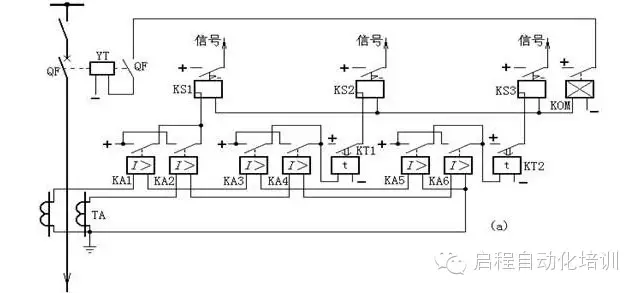
\includegraphics[width=\textwidth]{ti5.png}
    \caption{第~\ref{ti:5} 题的图}\label{fig:ti-5}
  \end{figure}
  \begin{solution}
    采用了三段式电流保护,由电流继电器、时间继电器、信号继电器、中间继电器、互感器、断路器、或门等元件组成。展开图见图~\ref{fig:ti-5-daan}。(参考课本P32)
    \begin{figure}
      \centering
      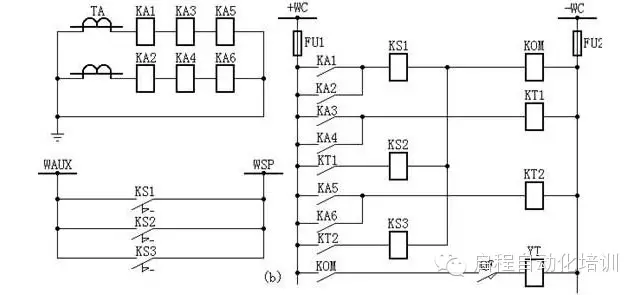
\includegraphics[width=\textwidth]{ti-5-daan.png}
      \caption{第~\ref{ti:5} 题的答案图}\label{fig:ti-5-daan}
    \end{figure}
  \end{solution}
  \item 依据电力元件正常工作、不正常工作和短路状态下的电气量幅值差异,已经构成哪些原理的保护,这些保护单靠保护整定值能求出保护范围内任意点的故障吗?
  \begin{solution}
    利用流过被保护元件电流幅值的增大,构成了过电流保护;利用短路时电压幅值的降低,构成了低电压保护;利用电压幅值的异常升高,构成了过电压保护;利用测量阻抗的降低和阻抗角的变大,构成了低阻抗保护。

    单靠保护增大值不能切除保护范围内任意点的故障,因为当故障发生在本线路末端与下级线路的首端出口时,本线路首端的电气量差别不大。所以,为了保证本线路短路时能快速切除而下级线路短路时不动作,这种单靠整定值得保护只能保护线路的一部分。
  \end{solution}
  \item 电力系统振荡为什么会使距离保护误动作?
  \begin{solution}
    电力系统振荡时,各点的电流、电压都发生大幅度摆动,因而距离保护的测量阻抗也在变化;当测量阻抗落入动作特性以内时,距离保护将发生误动作。
  \end{solution}
  \item 变压器差动保护不平衡电流是怎样产生的?
  \begin{solution}
    变压器励磁涌流的存在,变压器励磁电流(激磁电流)仅流经变压器的某一侧,因此通过电流互感器反应到差动回路中将形成不平衡电流。

    稳态运行时,变压器的励磁电流不大,只有额定电流的 2-\SI{5}{\percent}。在差动范围外发生故障时,由于电压降低,励磁电流减小。所以这两种情况下所形成的不平衡电流都很小,对变压器的差动保护影响不大。

    但是,当变压器空载投入和外部故障切除后电压恢复的情况下,则可能出现很大的励磁电流即励磁涌流。这个现象的存在是由于变压器铁心饱和及剩磁的存在引起的。
  \end{solution}
  \item \label{ti:t1-t6}如图~\ref{fig:t1-t6} 所示电网,装设方向过电流保护,保护采用两相不完全星形接线,方向元件按 $90^\circ$ 接线,试求:
  \begin{enumerate}
    \item 方向过电流保护的动作时限 $t_1\sim t_6$。
    \item 确定哪些保护应装设方向元件?
  \end{enumerate}
  \begin{figure}
    \centering
    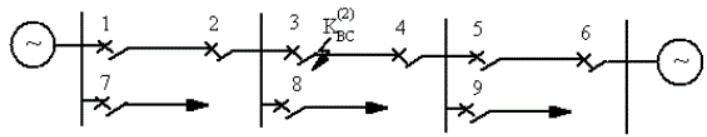
\includegraphics[width=\textwidth]{t1-t6.png}
    \caption{第~\ref{ti:t1-t6} 题的图}\label{fig:t1-t6}
  \end{figure}
  \begin{solution}
    \begin{enumerate}
      \item 设 $t_5 = \SI{0.5}{s}$,$t_7 = t_9 = \SI{1}{s}$,$t_8 = \SI{2}{s}$。
      那么 $t_3 = t_9 + \Delta t = 1 + 0.5 = \SI{1.5}{s}$,$t_1 = t_8 + \Delta t = 2 + 0.5 = \SI{2.5}{s}$,$t_2 = t_7 + \Delta t = 1 + 0.5 = \SI{1.5}{s}$,$t_4 = t_8 + \Delta t = 2 + 0.5 = \SI{2.5}{s}$,$t_6 = t_4 + \Delta t = 2.5 + 0.5 = \SI{3}{s}$。
      \item 保护2、3、5应装方向元件。
    \end{enumerate}
  \end{solution}
  \item 类似课本例题 2-9(然而考的时候题型并不一样——2020/06/19)。
\end{enumerate}
\end{document}